\chapter{O propósito do projeto}

\section{Contextualização}

\hspace{5mm} Cada vez mais percebe-se um aumento na quantidade de veículos a circular nas ruas das cidades - especialmente as grandes cidades. Esse alto volume de automóveis gera diversos problemas, tanto para a sociedade quanto para o meio ambiente.

\hspace{5mm} O tempo gasto pelas pessoas nos seus deslocamentos diários tem sido cada vez maior, o que diminui muito a sua qualidade de vida. Além disso, questões como poluição sonora e poluição do ar colocam em risco a saúde das pessoas e do planeta como um todo.

\hspace{5mm} Deste modo, a nossa empresa X analisou um dos grandes promotores deste problema: a não utilização inteligente dos recursos automóveis.

\hspace{5mm} A má utilização refere-se ao facto de maior parte dos automóveis que circulam nas estradas conterem muitos lugares, no entanto, apenas utilizados por poucas ou uma única pessoa.

\hspace{5mm} Segundo um estudo realizado nos Estados Unidos da América, as pessoas passam 75\% do tempo a conduzir sozinhas o seu carro.

\section{Objetivos do Projeto}

\hspace{5mm} Deste modo, a solução para este problema, foi a criação de uma aplicação que reúne pessoas que façam as mesmas deslocações, nos mesmos horários, e assim poderem partilhar um automóvel, dividr as despesas e ao mesmo tempo contribuir para o meio ambiente.

\hspace{5mm} Portanto, imagine-se um exemplo: A Maria tem um carro de cinco lugares, regista-se na aplicação e disponibiliza uma deslocação que irá fazer no dia 19 de Dezembro de 2019, de Braga até Lisboa, às \emph{9h00} e regressa às \emph{20h00} do mesmo dia. 

\hspace{5mm} O João e a Rita, são de Braga, pretendem ir a Lisboa nos mesmos horários que a Maria. Como estão todos  registados, a aplicação vai reuni-los para a partilha do automóvel, dividindo as despesas da deslocação. 

\hspace{5mm} Pontos positivos deste exemplo, evitou-se a má utilização de três veículos (Maria, João e Rita), reduz-se os preços da deslocação para cada um, e contribui-se para a redução da poluição para o meio ambiente e a quantidade de automóveis a circular pelas estradas. Pensando neste exemplo a larga escala, ou seja, milhares de utilizadores, a pouco e pouco, vai-se aproveitar melhor os recursos automóveis e por conseguinte reduzir as emissões prejudiciais ao ambiente.

\hspace{5mm} As figuras, seguintes (\ref{img:g1}, \ref{img:g2} e \ref{img:g3}), mostram as respostas às questões efetuadas nos inquéritos realizados aos alunos da Universidade do Minho. Nestes gráficos, podemos observar os problemas apresentados acima, dos quais a má utilização dos recursos automóveis, e os custos elevados com deslocações que poderia ser reduzido. O inquérito completo encontra-se em anexo.

\begin{figure}[H]
    \centering
	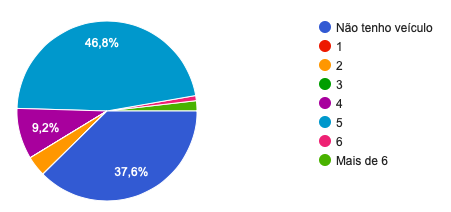
\includegraphics[scale=0.65]{imagens/g1.png}
	\caption{Respostas à questão "Quantos lugares tem o veículo que utiliza para as suas deslocações?".}
	\label{img:g1}
\end{figure}

\begin{figure}[H]
    \centering
	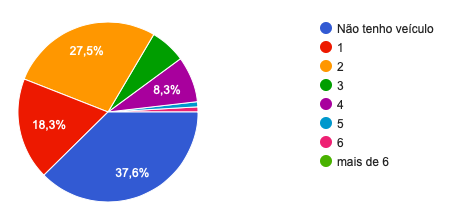
\includegraphics[scale=0.65]{imagens/g2.png}
	\caption{Respostas à questão "Quantos lugares em média são utilizados no seu automóvel?".}
	\label{img:g2}
\end{figure}

\begin{figure}[H]
    \centering
	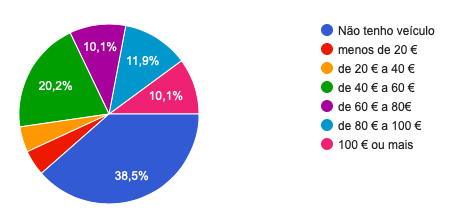
\includegraphics[scale=0.65]{imagens/g3.png}
	\caption{Respostas à questão "Qual a sua despesa mensal em combustível?".}
	\label{img:g3}
\end{figure}